\subsection{Visual Feedback with Attention Highlight on Musical Scores} \label{visualization_score}
\begin{figure}[h!]
  \centering
  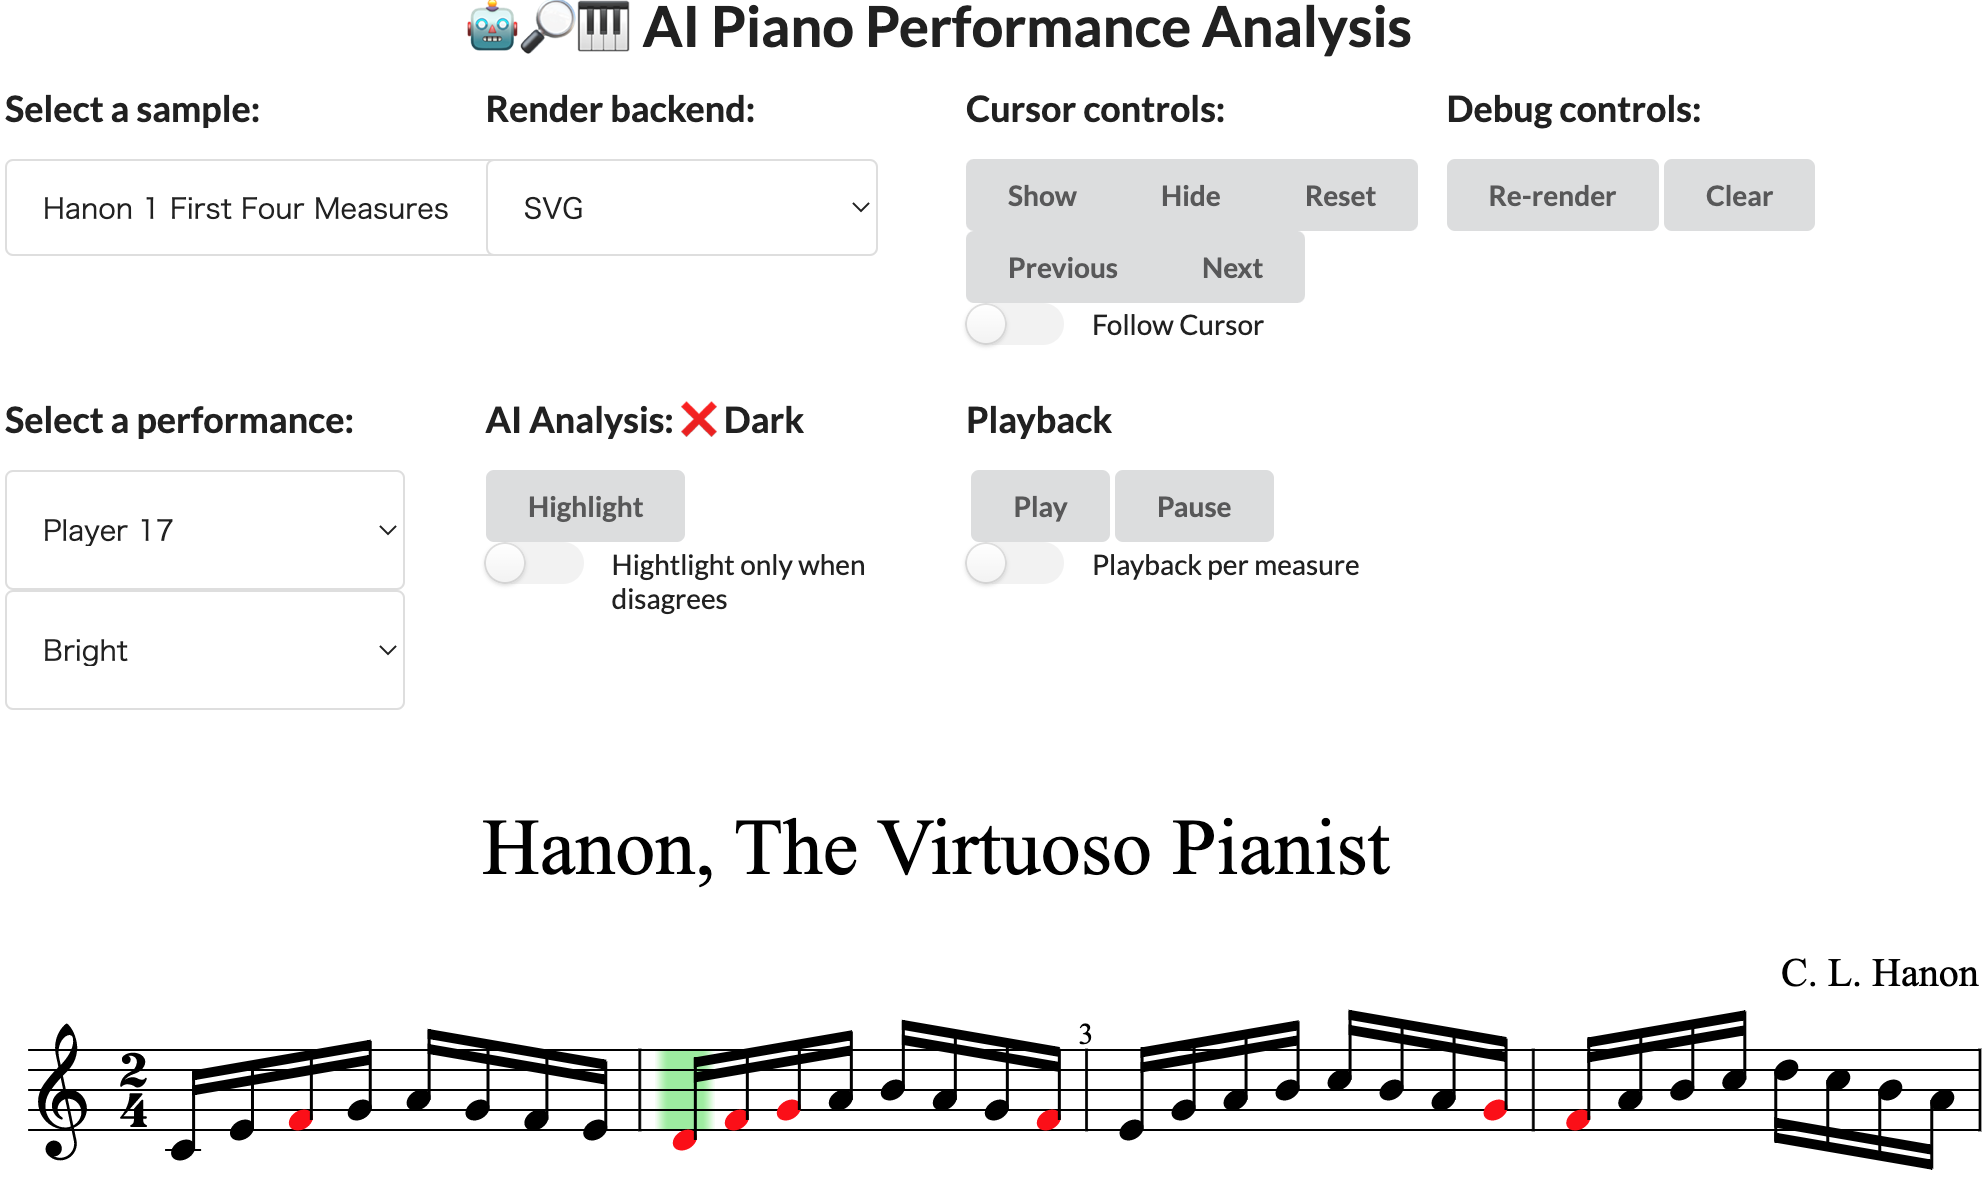
\includegraphics[width=\linewidth]{figures/UI_v110.png}
  \caption{Musical score based user interface based on our method. Music practitioners begin by selecting a performance to analyze, and then receive visual feedback by clicking the "Highlight" button. They can view the results of the performance analysis in the "AI Analysis" field, with the corresponding notes highlighted in red. By moving a green cursor to a highlighted note, practitioners can playback and review the performance from that point onward.}
  \Description{}
  \label{UI}
\end{figure}

We have demonstrated how the performance analysis model generates varying attention patterns and highlights important portions of a performance based on its analysis results. 
However, it is not a straightforward task to get insight into what kind of elements in the performance we have to discern and how to leverage the attention information to enhance the musical skills.

At this point, the recent technology to transcribe performance audio files into the MIDI format \cite{hawthorne2021, gardner2022} allows the analysis model to provide visual feedback on musical scores, with which most music practitioners are familiar to use.
We show an example of an user interface for the visual feedback on musical scores in Figure \ref{UI}.
This user interface of visual feedback on musical scores shows the analysis result in the "AI Analysis" field and provides the highlight information over the musical notes by highlighting them in red.

The musical score interface allows music practitioners to playback and review their performances by targeting at the musical notes with highlight. That is because the performance recording within which the attention highlights is aligned to the musical score.
For instance, they are able to use the musical score interface in the following manner:
\begin{enumerate}
   \item After their performance, check if they have performed in the correct way without anything wrong by clicking the "Highlight" button and obtaining the "AI Analysis" result.
   \item If there is something wrong in the performance, they will find the spot where the things are going wrong based on the highlight on the notes.
   \item Having identified where the things are wrong, they can move the cursor (colored in green in Figure \ref{UI}) and select the note,
   \item They playback and listen to the performance from the note they have selected and understand the important audio features.
   \item Based on the understanding, they perform again to see if they can improve their performance.
 \end{enumerate}
By repeatedly iterating through the steps above, music practitioners can gradually eliminate highlighted areas indicating errors or areas for improvement. 
Once all such highlights have been addressed, they will have effectively mastered the skill.

\begin{figure}[h!]
  \centering
  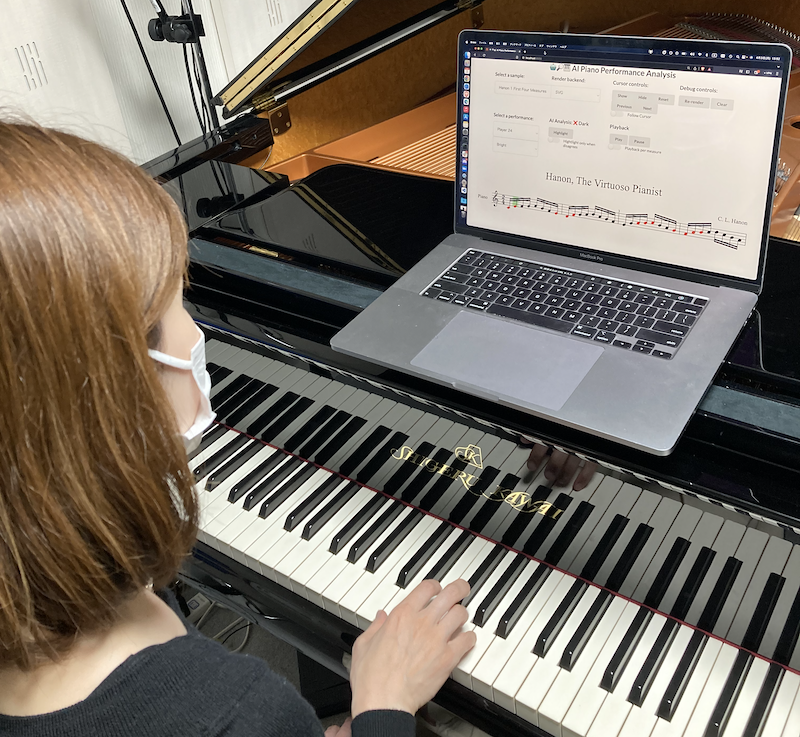
\includegraphics[width=\linewidth]{figures/system_usage_2224.png}
  \caption{Musical practitioners can utilize a system based on our method on any device equipped with standard web browsers, including laptops, tablets, and even smartphones.}
  \Description{}
  \label{system_usage}
\end{figure}

We note that the same method for highlight and playback within the musical score interface regarding musical brightness expression can be applied to other musical skills. 
Our method can offer visual feedback regarding additional skills through the interface, as long as the model assesses the skill with sufficient accuracy. 
For instance, if the model's accuracy in assessing general musical skills is comparable to its accuracy in assessing brightness expression, we can consider it a reliable reference for the musical skill.
It is then reasonable to derive highlights from its attention, and provide similar visual feedback on musical scores.